\documentclass[12pt]{article}

%-------------------------------------------------
%   THEMES & PACKAGES
%-------------------------------------------------
\usepackage{fancyhdr}
\usepackage{lastpage}
\usepackage{xcolor}
\usepackage{pdfpages}
\usepackage{hyperref}
\usepackage{graphicx}
\usepackage{float}
\usepackage{enumitem}
\usepackage{todonotes}
\usepackage{booktabs}
\usepackage{multirow}
\usepackage{gensymb}
\usepackage{pdfpages}

%%% Custom colors & commands
\newcommand{\HRule}[1]{\rule{\linewidth}{#1}}   % Horizontal rule

%-------------------------------------------------
%   COMMON INFO
%-------------------------------------------------
\newcommand{\hmwkTitle}{R \& D Proposal}
\newcommand{\hmwkTopic}{Learning Grasp Evaluation Models Using Synthetic 3D Object-Grasp Representations}
\newcommand{\hmwkDueDate}{December 15, 2017}
\newcommand{\hmwkClass}{Research and Development}
\newcommand{\hmwkAuthorName}{Minh H. Nguyen}
\newcommand{\hmwkAuthorSchool}{Bonn-Rhein-Sieg University of Applied Sciences}
\newcommand{\hmwkAdvisorFirst}{Prof. Dr. Paul G. Pl\"{o}ger}
\newcommand{\hmwkAdvisorSecond}{Alex Mitrevski}
\newcommand{\hmwkAdvisorThird}{Maximilian Sch\"{o}bel}

\graphicspath{{../images/}}
\renewcommand{\baselinestretch}{1.1}

%-------------------------------------------------
%   MARGINS
%-------------------------------------------------
\topmargin=-0.75cm
\evensidemargin=0cm
\oddsidemargin=0cm
\textwidth=16.0cm
\textheight=22.0cm
\headsep=0.6cm

%-------------------------------------------------
%   HEADERS & FOOTERS
%-------------------------------------------------
\pagestyle{fancy}
%-------------------------------------------------
% Special first page
\fancypagestyle{firststyle} {
    \fancyhf{}
    \fancyfoot{}
    \renewcommand\headrulewidth{0.pt}
    \renewcommand\footrulewidth{0.pt}
}
%-------------------------------------------------
\lhead{\hmwkAuthorName}
\rhead{\hmwkTitle}
%-------------------------------------------------
\cfoot{Page \thepage\ of \protect\pageref{LastPage}}
%-------------------------------------------------
\renewcommand\headrulewidth{0.4pt}
\renewcommand\footrulewidth{0.0pt}

%-------------------------------------------------
%   TITLE
%-------------------------------------------------
\title{\normalsize \textsc{\hmwkAuthorSchool}   % Subtitle
    \\[2.0cm]                                   % 2cm spacing
    \HRule{0.5pt} \\                            % Upper rule
    \LARGE \textbf{\uppercase{\hmwkTopic}}
    \HRule{2pt} \\ [0.5cm]                      % Lower rule + 0.5cm spacing
    \hmwkTitle\\[0.5cm]
    \normalsize \hmwkDueDate\\
}

\author{
    \\[4.0cm]
    Author:\\
    \hmwkAuthorName\\
    \ \\
    Advisors:\\
    \hmwkAdvisorFirst\\
    \hmwkAdvisorSecond\\
    \hmwkAdvisorThird\\
}

\date{}

%-------------------------------------------------
%   BIBLIOGRAPHY
%-------------------------------------------------
\usepackage[english]{babel}
\usepackage[backend=biber]{biblatex}
\addbibresource{../RnD.bib}
\addbibresource{proposal.bib}

%-------------------------------------------------
%   BEGIN
%-------------------------------------------------
\begin{document}
%-------------------------------------------------
    \maketitle
    \thispagestyle{firststyle}
    \newpage

%-------------------------------------------------
\section{Introduction}

    %---------------------------------------------
    \subsection{Motivation}
    Finding a suitable grasp strategy for a given object is a challenging problem, especially in the area of service robotics where the query objects are usually unknown or not fully known beforehand, the viewing point of objects changes as the robot moves, and objects oftentimes need to be grasped in a certain way to perform specific tasks. Grasp synthesis is generally divided into analytical and empirical approaches \cite{Bohg2014,Sahbani2012}. Analytic methods often optimize some metrics which measure one or multiple properties of a robotic hand, namely dexterity, object equilibrium and stability, or the ability to exhibit a certain dynamic behavior \cite{Bohg2014}. However, these methods often make assumptions about the object (i.e. shapes or poses) and therefore are prone to errors and do not generalize well to novel objects, while taking more time to match point clouds to known models \cite{Goldfeder2011}. Empirical or data-driven approaches generally sample from several grasp candidates and rank them according to a specific metric, which can be found heuristically or generated in simulation and on real robots \cite{Bohg2014}. These approaches do not rely on objects' physical model and therefore can generalize better to familiar or unknown objects compared to analytical approaches. Furthermore, learning to grasp via mimicking human grasping eliminates the need for task modeling. However, data collection for these methods is often tedious and costly \cite{mahler2017}.

	Mahler et al. \cite{mahler2017} proposed a pipeline to generate synthetic data (Dex-net 2.0) for training Grasp Quality Convolutional Neural Network (GQ-CNN), a model which can rapidly predict probability of successful grasp from depth image. Despite achieving high precision in successful grasp prediction, the model is limited in how grasps are represented: the grasp's approach vector and camera view point is presumed to be perpendicular to the table, while the gripper configuration and wrist orientation used as training input are simplified to the angle of the parallel-jaw grasp axis with respect to the table. The model is therefore insufficient for use with mobile robots, where the camera pose often changes as the robot moves, and the grasp approach vector is not known beforehand.

    This research aims to extend the work by Mahler et al. \cite{mahler2017} for use in mobile robotics, specifically on the Care-O-bot 3 platform \footnote{\url{https://www.care-o-bot.de/en/care-o-bot-3.html}}, through synthesizing a new dataset using a more general grasp representation and training a new CNN model on this dataset.

    %---------------------------------------------
    \subsection{Prior Work}

    Figure \ref{fig:grasp_synthesis_mind_map} maps the different aspects that may affect generation of grasp hypotheses. As applied to a specific use case to be described in section \ref{use-case}, the proposed approach will focus on 3D object features and synthesizing grasp candidates for familiar objects. Section \ref{hw-spec} will describe the robot platform, including arm and gripper configuration. This section will focus on surveying literature about object-grasp representation, 3D grasp synthesis, 3D grasp quality metrics, and task compatibility. In the final part, a description of the Dex-net data generation process will be included.

    \begin{figure}[H]
        \centering
        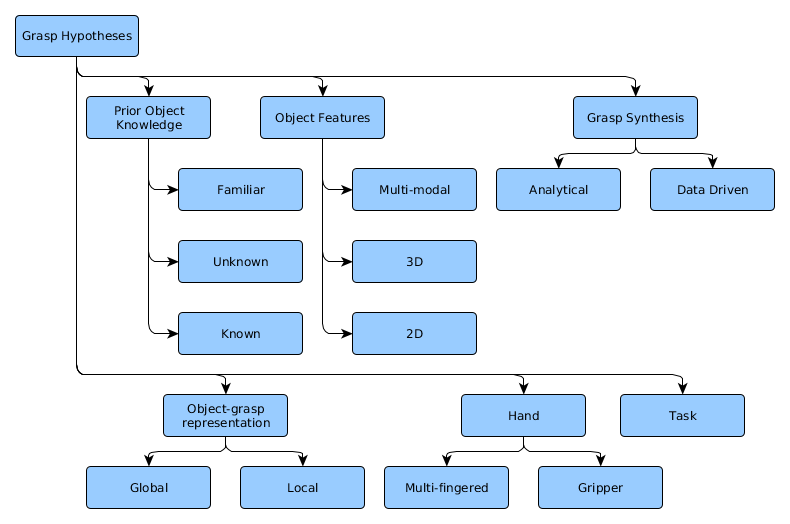
\includegraphics[width=0.7\textwidth]{bohg14-grasp_synthesis_mind_map}
        \caption{Aspects which may influence generation of grasp hypotheses \cite{Bohg2014}.}
        \label{fig:grasp_synthesis_mind_map}
    \end{figure}

    \subsubsection{Object-Grasp representation}
    Bohg et al. \cite{Bohg2014} parameterized grasps as
    \begin{itemize}
        \item the \emph{grasping point} of the object where the gripper should be aligned,
        \item an \emph{approach vector} from which the gripper shall approach the \emph{grasping point},
        \item the \emph{wrist orientation} of the robotic hand,
        \item and an \emph{initial gripper configuration}.
    \end{itemize}
    The article also categorized object-grasp representation approaches into ones which extract local (i.e. curvature, contact area with the hand) or global features (center of mass, bounding box). In generating Dex-net 2.0, Mahler et al. represent grasps in 2D images by aligning the image center to the gripper central point and the image's middle row to the grasp axis \cite{mahler2017}. In general, however, object-grasp representation is highly dependent on the specific hardware setup (i.e. the robot arm and gripper).

    \subsubsection{3D grasp synthesis}

    One of the key element of grasping strategies is stability. As defined in \cite{Roa2015}, a grasp is stable if position error of object caused by a disturbance disappears after the disturbance vanishes. Two important subsets of stable grasps are \emph{force closure} and \emph{form closure}. For a force closure grasp, all fingers can apply force on object to produce wrenches in all directions. A grasp that can achieve force closure with frictionless point contacts achieves form closure \cite{Sahbani2012}.

    Grasp synthesis is generally categorized into analytical and empirical approaches: analytical methods (figure \ref{fig:analytic_grasp}) rely on geometric, kinematic and/or dynamic formulations, while empirical ones (figure \ref{fig:empirical_grasp}) generally build a knowledge base of grasp experience for sampling grasp candidates and rank them based on some quality metric \cite{Sahbani2012,Bohg2014}.

    \begin{enumerate}
        \item Analytical approaches are categorized in \cite{Sahbani2012} into methods which compute force-closure grasps and ones which consider task compatibility. Force-closure methods are further divided into methods which synthesize force-closure grasps and methods which attempt to find an optimal force-closure grasp using a grasp quality metric. Su\'{a}rez reviewed grasp quality metrics extensively in \cite{suarez2006}, and a more recent review was done by Roa and Su\'{a}rez in \cite{Roa2015}.
        \item While Sahbani et al. categorized empirical approaches into techniques which focus on human observation and ones focusing on object observation \cite{Sahbani2012}, Bohg et al. argued that sorting these techniques based on the assumption of what is known about the query objects would better capture the diversity of the techniques \cite{Bohg2014}. Empirical approaches are thus divided in the latter article into ones which deal with known, familiar or unknown objects.
    \end{enumerate}

    \begin{figure}[H]
        \centering
        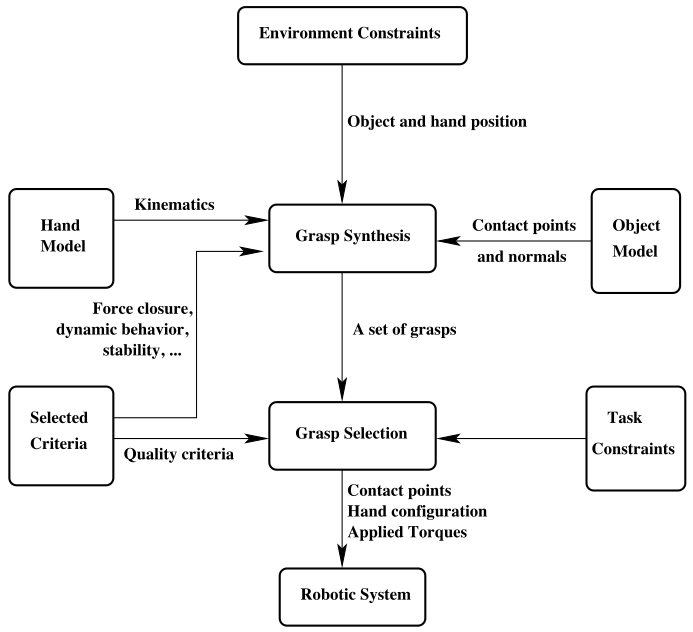
\includegraphics[width=0.65\textwidth]{sahbani12-analytic_grasp_strategy}
        \caption{Grasp synthesis using analytical approaches \cite{Sahbani2012}.}
        \label{fig:analytic_grasp}
    \end{figure}

    \begin{figure}[H]
        \centering
        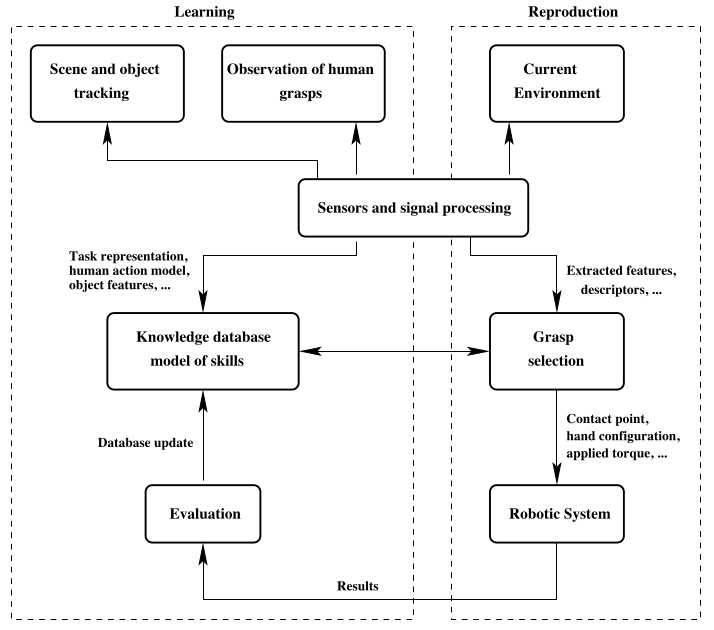
\includegraphics[width=0.65\textwidth]{sahbani12-empirical_grasp_strategy}
        \caption{Grasp synthesis using empirical approaches \cite{Sahbani2012}.}
        \label{fig:empirical_grasp}
    \end{figure}

    \subsubsection{3D grasp quality metrics}

    \begin{table}[H]
        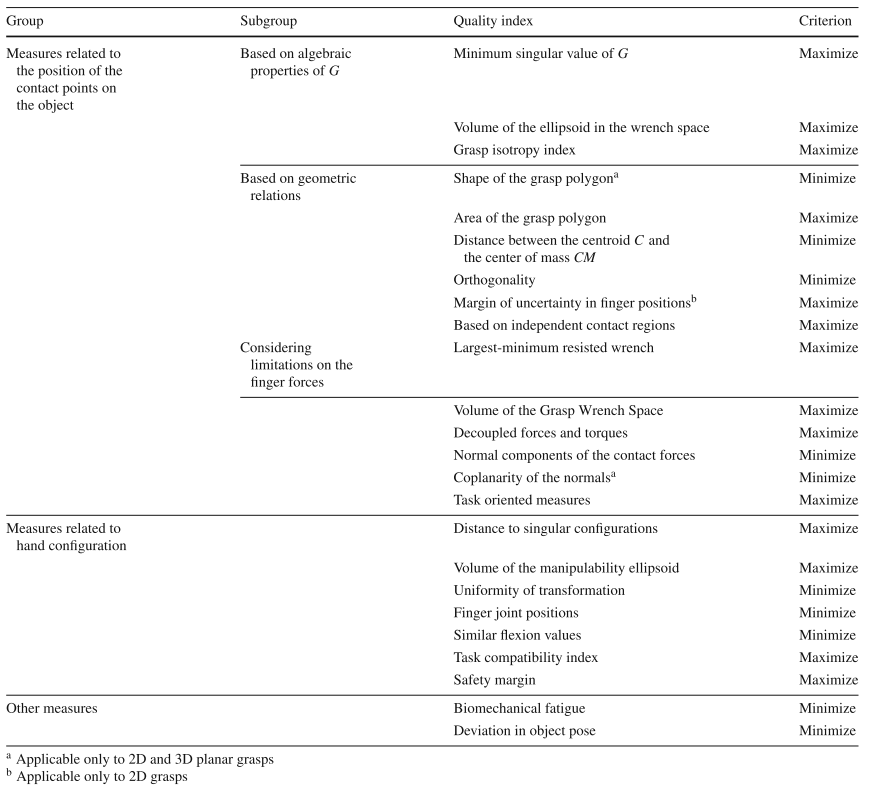
\includegraphics[width=\textwidth]{roa_suarez-2015-grasp_metrics}
        \caption{Grasp quality measures \cite{Roa2015}.}
        \label{table:grasp_metric}
    \end{table}

    Roa and Su{\'a}rez group grasp quality measures into approaches focusing on contact point position, hand configuration, and ones which combine both metric types \cite{Roa2015}.
    \begin{itemize}
        \item Contact point grasp quality measures focus on the object's properties, friction constraints and form/force closure conditions.
        \item Hand configuration measures focus on studying the properties of the hand-object Jacobian $H$.
        \item Grasp measures can be combined serially or in parallel to capture different aspects of a grasp's quality. In the serial approach, one quality measure is applied to find several grasp candidates, then another metric is used to choose the optimal candidate. The parallel approach combines the different measures in a single global index.
    \end{itemize}
    Table \ref{table:grasp_metric} illustrates how contact point and hand configuration related approaches can be further categorized into subgroups, and include metrics based on bio-mechanical fatigue and deviation of object pose which are not encapsulated by the aforementioned groups.

    %\subsubsection{Convolutional Neural Network as feature extractor for point clouds}

    \subsubsection{Task Compatibility}
    In addition to stability, a successful grasping strategy also has to take into account the task to be performed with the grasped object. However, Sahbani et al. \cite{Sahbani2012} points out that incorporating task compatibility in to grasp synthesis, is still an open challenge because of the difficulty in modeling a task and the computational cost of finding a suitable grasp once a task is defined. These challenges are particularly relevant to analytic grasp synthesis, but is also not solved by empirical approaches. Methods which mimic human grasping alleviate the need for modeling tasks but is not fully automatic when facing new objects, while methods based on object observations have to generate many grasp candidates and face the same difficulty of task modeling as analytical approaches. One possible approach suggested by the article is to directly identify object features that are relevant to the requested tasks. Approaches to task modeling include methods based on manipulability ellipsoids \cite{Yoshikawa1990} and task space polytopes \cite{lee1997}, or building a task compatibility index measuring the similarity between the optimal directions of the manipulator and the movements required by a specific task \cite{chiu1988}.

    \subsubsection{Dex-Net 2.0 Data Generation} \label{dexnet-generation}
    \begin{itemize}
        \item Compute stable object poses from 3D mesh models from Dex-Net 1.0 \cite{mahler2016}, object meshes are rescaled to fit within the gripper physical constraints, and store poses with probability of occurrence above a threshold.
        \item Grasps are sampled using rejection sampling to ensure coverage of the object surface, ranked and selected using a grasp quality metric.
        \item 2D images are generated from grasp candidates as training data with the antipodal axis aligned to the middle row of the image.
    \end{itemize}

    %---------------------------------------------
    \subsection{Hardware Specification} \label{hw-spec}
    The robot platform to be used for experimentation is the Care-o-bot 3 from Fraunhofer Institute for Manufacturing Engineering and Automation \footnote{\url{https://www.ipa.fraunhofer.de/}}, mounted with a Schunk SDH \footnote{\url{https://schunk.com/de_en/gripping-systems/series/sdh/}} gripper and an ASUS Xtion PRO RGB-D camera \footnote{\url{https://www.asus.com/3D-Sensor/Xtion_PRO/}}.

    \begin{table}[H]
        \centering
        \begin{tabular}{lr}
            \toprule
            Specification name & Value \\ \midrule
            Number of fingers & 3 \\
            Maximum admissible finger length (mm) & 155 \\
            Finger distance (mm) & 66 \\
            Degrees of freedom & 7 \\
            Degrees of freedom per finger & 2 \\
            Degrees of freedom 2-finger-rotation & 1\\
            \bottomrule
        \end{tabular}
        \caption{Schunk SDH gripper specifications.}
    \end{table}

    \begin{table}[H]
        \centering
        \begin{tabular}{lr}
            \toprule
            Specification name & Value \\ \midrule
            \multirow{2}{*}{Depth image size} & VGA (640x480) : 30fps \\
                                              & QVGA (320x240): 60fps \\
            Maximum admissible finger length (mm) & 155 \\
            Field of view (Horizontal, Vertical, Diagonal) & 58\degree H, 45\degree V, 70\degree D \\
            Distance of use & Between 0.8m and 3.5m \\
            \bottomrule
        \end{tabular}
        \caption{ASUS Xtion PRO depth camera specifications.}
    \end{table}

    %---------------------------------------------
    \subsection{Use Case} \label{use-case}
    This project aims at the manipulation tasks relevant to the Robocup@Home competition \footnote{\url{http://www.robocupathome.org/}}, i.e. picking up and transporting household objects directly or with containers, opening doors, etc. Figure \ref{fig:robocup_objects} shows typical objects that the robot need to grasp at the competition. There are five main object groups \cite{vanBeek17}:
    \begin{itemize}
    	\item Known objects: artificial and regular-shaped objects which are provided before competition for training.
    	\item Alike objects: slightly different from known objects (i.e. in color or shapes), also provided before competition.
    	\item Containers: objects which can be used for storage, pouring or transport such as trays or bowls.
    	\item Special objects: requires special handling to accomplish a specific task. Examples are door handles, chairs, or walking sticks. Samples of these objects will not be provided before competition.
    	\item Unknown objects: any objects that are unknown beforehand but can be grasped or handled.
    \end{itemize}
    \begin{figure}[H]
    	\centering
    	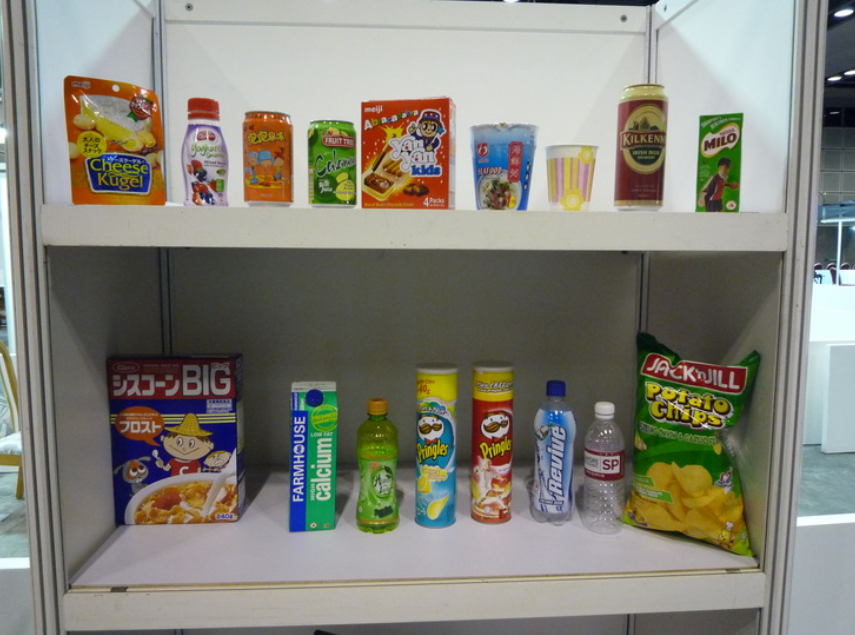
\includegraphics[width=0.65\textwidth]{vanBeek17-robocup_objects}
    	\caption{Typical objects at the Robocup@Home competition \cite{vanBeek17}.}
    	\label{fig:robocup_objects}
    \end{figure}

    %---------------------------------------------
    \subsection{Approach}
    \begin{itemize}
        \item Define grasp plan representation in 3D.
        \item Choose a (or several) grasp synthesis strategy to generate grasp candidates.
        \item Choose a grasp quality metric for rating synthesized grasp candidates.
        \item Generate synthetic 3D object-grasp representations following the Dex-Net 2.0 data generation process \cite{mahler2017}.
        \item Train a neural networks model on the synthesized data to calculate a quality measure for possible grasp candidates given an object.
    \end{itemize}

    %---------------------------------------------
    \subsection{Expected Results}
    \begin{itemize}
    	\item At minimum the project should result in a pipeline to generate training data for a model which can rapidly evaluate grasp candidates synthesized for detected objects.
    	\item An extension to the project is implementing a full grasp planner for testing on the Care-o-bot platform, including object detection, grasp synthesis, grasp candidate ranking, and grasp execution.
    	\item A stretch goal of the project is to incorporate task compatibility in the data generation pipeline.
    \end{itemize}


%-------------------------------------------------
\section{Project Plan}

    %---------------------------------------------
    \subsection{Work Packages}
    \begin{itemize}
    	\item Literature research
    	\item Choose an approach to represent object-grasp in point clouds and implement generation of this representation using point cloud data.
    	\item Choose a grasp synthesis algorithm and generate synthesized grasps with the implemented object-grasp representation.
    	\item Choose and implement a grasp quality metric for ranking synthesized grasp candidates.
    	\item Synthesize training data for grasp quality model:
    	\begin{itemize}
    		\item from a data set of 3D object models, generate point clouds from various view points of objects in various poses,
    		\item generate grasp candidates using the chosen object-grasp representation method,
    		\item and calculate grasp quality using the chosen metric.
    	\end{itemize}
    	\item Train a model which can calculate grasp quality from grasp candidates synthesized for a detected object.
    	\item Implement a grasp planner on the robot platform to test the trained model.
    	\item Writing report.
    \end{itemize}

    %---------------------------------------------
    \subsection{Work Schedule}
    \begin{figure}[H]
    	\centering
    	\setlength{\fboxsep}{0pt}
    	\fbox{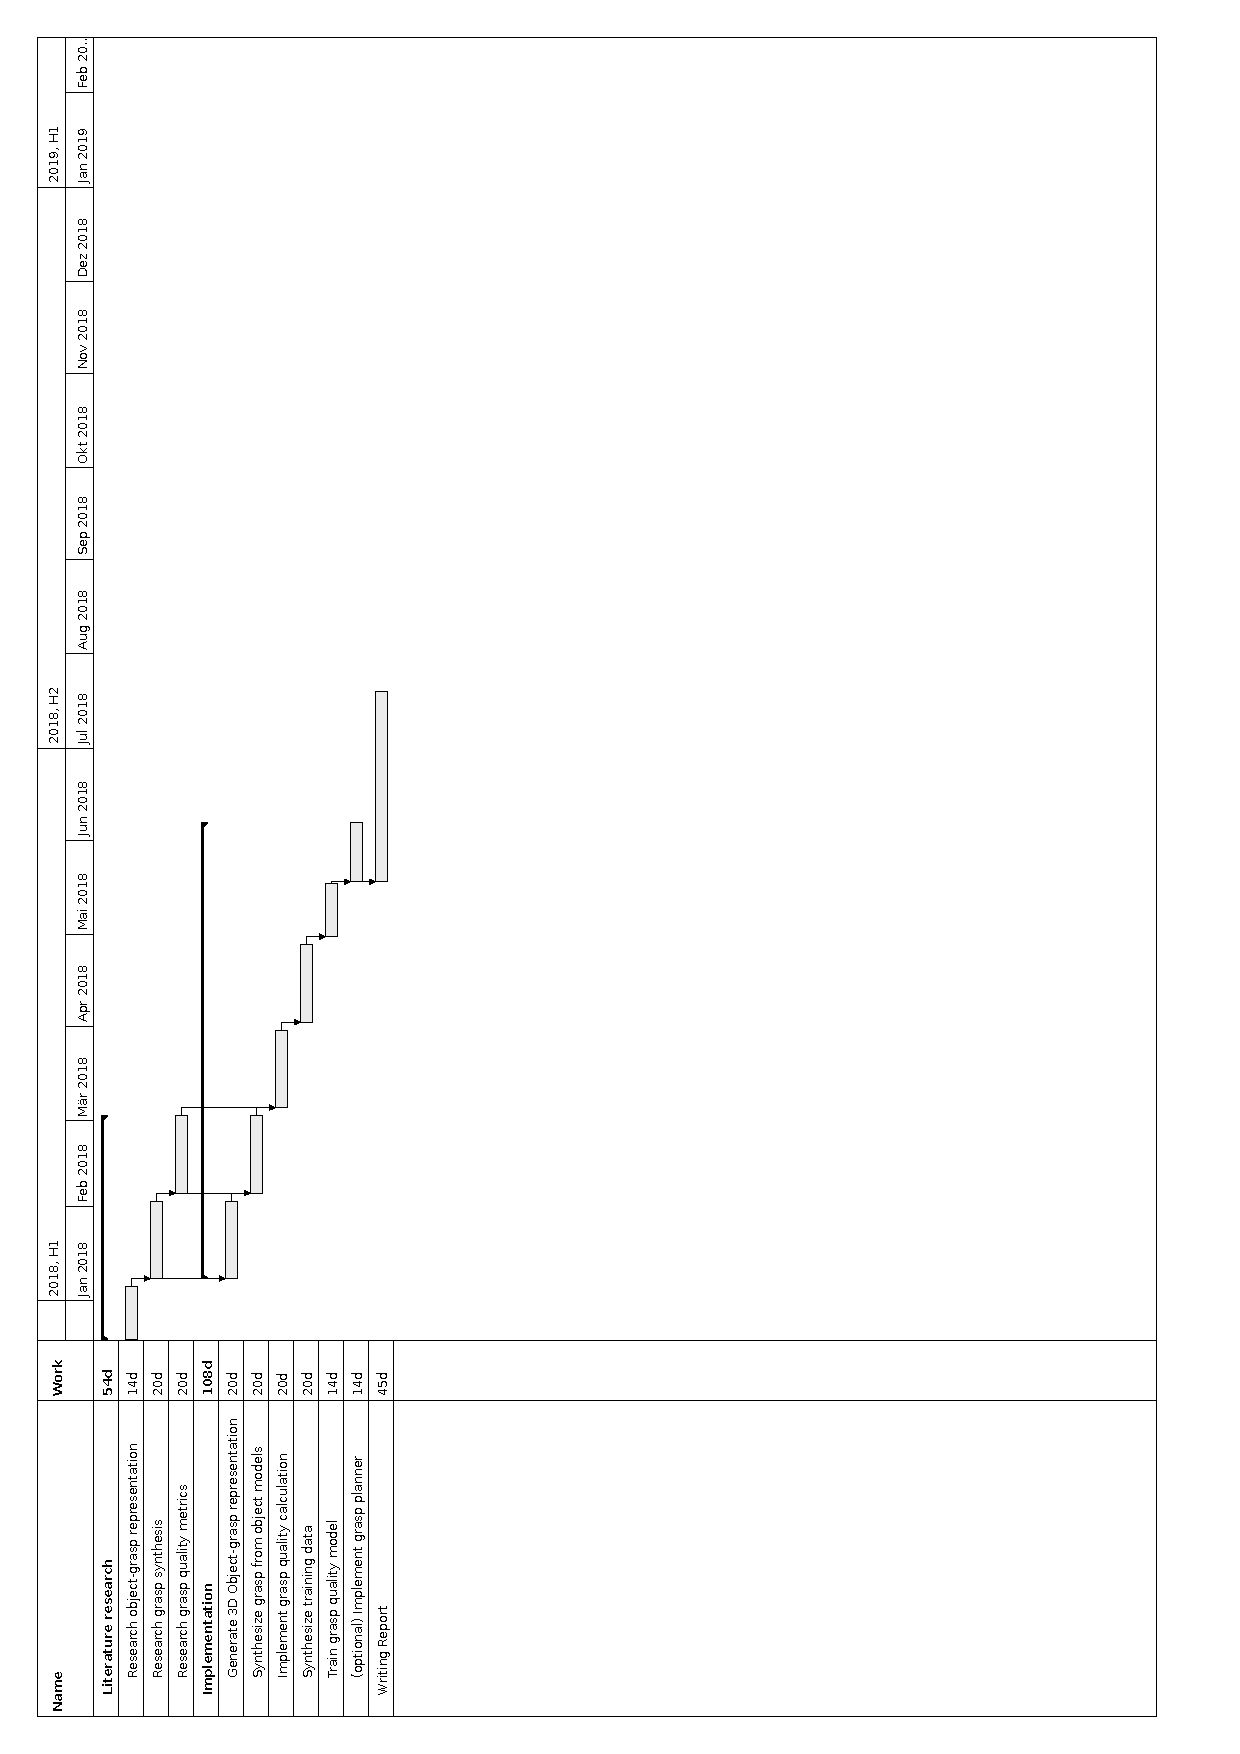
\includegraphics[width=\textwidth]{project_plan}}
    	\caption{Project Gantt Chart.}
    	\label{fig:project_plan}
    \end{figure}

	\pagebreak
	\printbibliography

%-------------------------------------------------
%   END
%-------------------------------------------------
\end{document}
